% Options for packages loaded elsewhere
\PassOptionsToPackage{unicode}{hyperref}
\PassOptionsToPackage{hyphens}{url}
\PassOptionsToPackage{dvipsnames,svgnames,x11names}{xcolor}
\PassOptionsToPackage{space}{xeCJK}
\documentclass[
  10pt,
]{article}
\usepackage{xcolor}
\usepackage[margin=0.65in]{geometry}
\usepackage{amsmath,amssymb}
\setcounter{secnumdepth}{-\maxdimen} % remove section numbering
\usepackage{iftex}
\ifPDFTeX
  \usepackage[T1]{fontenc}
  \usepackage[utf8]{inputenc}
  \usepackage{textcomp} % provide euro and other symbols
\else % if luatex or xetex
  \usepackage{unicode-math} % this also loads fontspec
  \defaultfontfeatures{Scale=MatchLowercase}
  \defaultfontfeatures[\rmfamily]{Ligatures=TeX,Scale=1}
\fi
\usepackage{lmodern}
\ifPDFTeX\else
  % xetex/luatex font selection
  \setmainfont[]{Arial}
  \setmonofont[]{Consolas}
  \ifXeTeX
    \usepackage{xeCJK}
    \setCJKmainfont[]{Microsoft YaHei}
  \fi
  \ifLuaTeX
    \usepackage[]{luatexja-fontspec}
    \setmainjfont[]{Microsoft YaHei}
  \fi
\fi
% Use upquote if available, for straight quotes in verbatim environments
\IfFileExists{upquote.sty}{\usepackage{upquote}}{}
\IfFileExists{microtype.sty}{% use microtype if available
  \usepackage[]{microtype}
  \UseMicrotypeSet[protrusion]{basicmath} % disable protrusion for tt fonts
}{}
\makeatletter
\@ifundefined{KOMAClassName}{% if non-KOMA class
  \IfFileExists{parskip.sty}{%
    \usepackage{parskip}
  }{% else
    \setlength{\parindent}{0pt}
    \setlength{\parskip}{6pt plus 2pt minus 1pt}}
}{% if KOMA class
  \KOMAoptions{parskip=half}}
\makeatother
\usepackage{longtable,booktabs,array}
\usepackage{calc} % for calculating minipage widths
% Correct order of tables after \paragraph or \subparagraph
\usepackage{etoolbox}
\makeatletter
\patchcmd\longtable{\par}{\if@noskipsec\mbox{}\fi\par}{}{}
\makeatother
% Allow footnotes in longtable head/foot
\IfFileExists{footnotehyper.sty}{\usepackage{footnotehyper}}{\usepackage{footnote}}
\makesavenoteenv{longtable}
\usepackage{graphicx}
\makeatletter
\newsavebox\pandoc@box
\newcommand*\pandocbounded[1]{% scales image to fit in text height/width
  \sbox\pandoc@box{#1}%
  \Gscale@div\@tempa{\textheight}{\dimexpr\ht\pandoc@box+\dp\pandoc@box\relax}%
  \Gscale@div\@tempb{\linewidth}{\wd\pandoc@box}%
  \ifdim\@tempb\p@<\@tempa\p@\let\@tempa\@tempb\fi% select the smaller of both
  \ifdim\@tempa\p@<\p@\scalebox{\@tempa}{\usebox\pandoc@box}%
  \else\usebox{\pandoc@box}%
  \fi%
}
% Set default figure placement to htbp
\def\fps@figure{htbp}
\makeatother
\setlength{\emergencystretch}{3em} % prevent overfull lines
\providecommand{\tightlist}{%
  \setlength{\itemsep}{0pt}\setlength{\parskip}{0pt}}
\usepackage{bookmark}
\IfFileExists{xurl.sty}{\usepackage{xurl}}{} % add URL line breaks if available
\urlstyle{same}
\hypersetup{
  colorlinks=true,
  linkcolor={Maroon},
  filecolor={Maroon},
  citecolor={Blue},
  urlcolor={blue},
  pdfcreator={LaTeX via pandoc}}

\author{}
\date{}

\usepackage{float}
\usepackage{needspace}
\Urlmuskip=0mu plus 2mu\relax
\renewcommand{\figurename}{图}
\begin{document}

\section{数据整合、退化算法审计与新一轮训练结果}\label{ux6570ux636eux6574ux5408ux9000ux5316ux7b97ux6cd5ux5ba1ux8ba1ux4e0eux65b0ux4e00ux8f6eux8badux7ec3ux7ed3ux679c}

2026年11月13日 · Eye Sentinel

\href{training-results.en.md}{English} ·
\href{training-results.zh.pdf}{中文PDF} ·
\href{../progress-overview.zh.md}{当日进度总览}

\subsection{本轮完成了什么}\label{ux672cux8f6eux5b8cux6210ux4e86ux4ec0ux4e48}

本报告承接同日的\href{../data-review/data-and-degradation-review.zh.md}{数据与退化方法审查}，记录审计后的数据划分、四组训练和开发集评价；\href{../experimental-analysis/experimental-analysis.zh.md}{实验分析}进一步解释来源差异、训练采样和选模的影响。

新增数据与原疾病数据合并为固定版本 expanded\_20261113。四组
EfficientNet-B0 使用相同的 ImageNet
预训练初始化，分别比较原数据、扩展数据、扩展数据加30\%退化和扩展数据加50\%退化。每组完成1,200次优化更新，即1,200次实际参数调整；配置中的20轮是训练上限，本轮按更新次数结束。模型验证集用于选择权重，规则开发集用于分析表现和后续设计人工复核规则，两者用途分开。四组均使用随机种子20261113。

AUROC的全称是受试者工作特征曲线下面积。随机抽取一张阳性和一张阴性照片时，它表示模型给阳性更高分的概率，并列分数计一半。0.5对应随机排序，1对应完全区分；例如0.93表示约93\%的阳性／阴性配对中阳性分数更高。具体筛查阈值下的漏诊和误报另行评价。

下面首先报告各组由模型验证集选中的权重：扩展无退化组为第300次更新，其余组为第1,200次更新。相同第1,200次更新的比较见``模型选择的补充检查''，也用于当日总览和实验分析。

在305张ODIR规则开发图像（28张正例）上，原数据与扩展数据方案的AUROC分别为
0.9712 和 0.9323；30\%和50\%退化方案分别为 0.9281 和
0.9404。在12张真实低质量正例上，以0.5为展示阈值，四组漏诊数依次为 5, 0,
0,
0。这组结果表明，扩展数据提高了这12张低质量阳性的检出，同时降低了ODIR原图的排序表现。下文分别报告来源结果、漏诊与误报，以解释这两种变化。

在153张KEH视盘裁剪开发图像（75张正例）上，四组AUROC依次为 0.6627,
0.9212, 0.9321,
0.9368。KEH图像主要是视盘局部裁剪，与完整眼底照片有不同的成像范围。ODIR的28张阳性照片属于19个已确认阳性关联组；一组内的双眼或关联图像在统计时共同处理。

\subsection{数据整合和本次新增发现}\label{ux6570ux636eux6574ux5408ux548cux672cux6b21ux65b0ux589eux53d1ux73b0}

统一疾病清单共有24,491张图像。文件SHA256用于核对图像内容是否变化；完整RGB解码检查确认图像可以读取。全部图像通过检查，新增9,070张与审查阶段记录的原始像素一致。按患者、同眼、同图变体及已确认跨来源关联合并分组后，关联组跨用途和跨用途相同RGB像素均为零。386个已知患者标识均分配到单一用途。缺少患者标识的来源按已确认图像关系分组，所记录的关联组数是图像分组数。

独立重建关联图发现，原疾病数据中有18张图像与官方EyeQ测试组关联。本次从新版本排除16张训练图和2张模型验证图，并落实12张原规则开发图的既有修复。这18张图的移除同时应用于原数据对照和三个扩展组。历史模型在移除前训练；涉及这些EyeQ组的后续评价使用本轮模型。

\Needspace{12\baselineskip}
\begin{longtable}[]{@{}lrrr@{}}
\toprule\noalign{}
用途 & 原数据图像／正例 & 新增图像／正例 & 合计图像／正例 \\
\midrule\noalign{}
\endhead
\bottomrule\noalign{}
\endlastfoot
训练 & 10,338 / 4,409 & 5,142 / 1,996 & 15,480 / 6,405 \\
模型验证 & 1,188 / 487 & 858 / 336 & 2,046 / 823 \\
规则开发 & 1,220 / 503 & 833 / 311 & 2,053 / 814 \\
内部及新增保留测试 & 1,233 / 489 & 2,237 / 803 & 3,470 / 1,292 \\
\end{longtable}

另保留ACRIMA的705张、396张正例和HYGD的737张、540张正例。PAPILA全来源420张（87张正例，来自47名已知阳性患者）纳入保留测试，105张官方测试图沿整组传播为测试用途。204张疑似图单独保存，疾病二分类监督使用有明确阳性或阴性标签的图像。LAG、GRAPE、FIVES、Fundus-AVSeg和MSHF按已确认关联联合分组。KEH保留视盘裁剪域说明；RG转诊标签与各来源临床诊断标签保持分列。

真实低质量正例分别保留在训练72张、模型验证12张、规则开发12张、测试50张。FIVES按至少一个官方质量维度差定义，MSHF按官方总体质量编码0定义，两者不合并成同一种质量标注。规则开发的12张是FIVES
7张和MSHF 5张。

\begin{figure}[H]
\centering
\pandocbounded{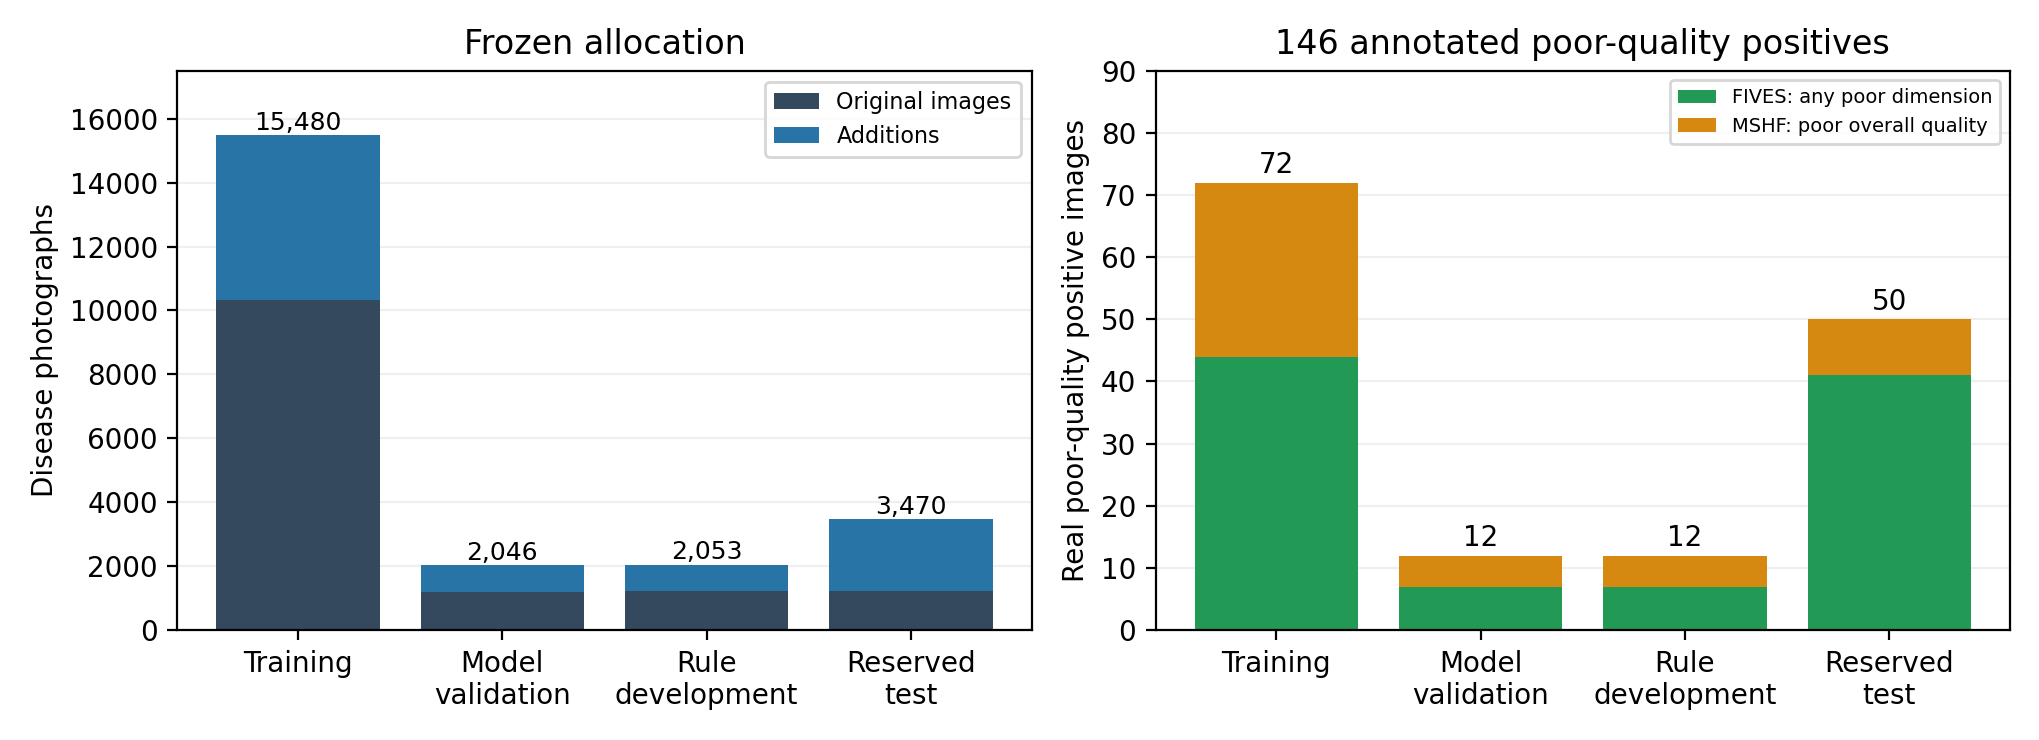
\includegraphics[keepaspectratio,alt={冻结数据划分与真实低质量阳性分布}]{cohort-and-quality.png}}
\caption{冻结数据划分与真实低质量阳性分布}
\end{figure}

图1左侧按用途区分原数据和新增数据，合计包含训练、验证、开发和内部及新增保留测试；ACRIMA和HYGD的外部测试单列于正文。右侧显示146张真实低质量阳性按用途和来源的分布。FIVES与MSHF采用各自的官方质量定义。

\subsection{退化算法与作者模型}\label{ux9000ux5316ux7b97ux6cd5ux4e0eux4f5cux8005ux6a21ux578b}

已下载CoFe-Net、ArcNet、FD3、Catintell和CUNSB-RFIE五个固定提交版本，核查压缩包完整性、代码、许可和权重。CUNSB-RFIE的G、D、E、F四份权重均可用受限权重加载方式读取，张量均为有限值；G严格匹配作者DSCNet，并完成一次320×320
CPU前向运行。这次运行核实了权重和作者代码的相容性。作者网络用于图像恢复，本轮疾病训练的退化图则由项目实现的成像模拟生成；两者是不同处理步骤。

退化增强在疾病图补边并缩放到320×320后、ImageNet标准化前施加。每次等概率选择照明变化、失焦或轻度散射中的一种；失焦可附带轻噪声或JPEG压缩。散射通过平滑亮度混合降低局部对比度。模糊大小按有效眼底视野直径换算，曝光范围0.72--1.12，512像素视野参考模糊半径0.5--2.0，散射透明度0.03--0.10。图像标识、轮次和随机种子决定参数；保存的参数可重新生成相同图像，原始黑边保持原值。退化概率与疾病标签无关。

18对HRF同眼重拍及120对Real
Fundus的描述性比对显示，真实低／高质量绿通道Laplacian方差比中位数分别约0.516和0.101，而固定温和失焦例约0.805和0.719。这一方差描述边缘和细节的变化，也受噪声、图像对齐和内容影响；本次比对用于说明训练退化的强度。对质量模型的监督仍使用原图及其教师质量分数或人工质量等级，合成退化只用于疾病训练。

\subsection{训练预算、采样和模型选择}\label{ux8badux7ec3ux9884ux7b97ux91c7ux6837ux548cux6a21ux578bux9009ux62e9}

四组共享清单、验证角色、种子20261113、320像素输入、batch
16、AdamW学习率0.0001和相同更新预算。原数据组只过滤训练来源，不改变验证集。每张图的抽样权重为其来源、类别组合图像数的平方根倒数；图像数较少的组合因此获得更高的单图抽样概率。四组使用同一规则，扩展组加入来源后，各原来源获得的训练采样次数会改变。累计抽到的不同原始图像依次为
8339, 9830, 9830, 9830，这些计数与生成版本数分开保存。实际退化抽样比例为
30.1\% 和 50.1\%。

每300次更新验证一次，按11个同时有正负例的来源各自AUROC的平均值选权重。来源AUROC先分别计算，再等权平均。恢复训练和多进程加载的一致性核验见配套审计记录。

\Needspace{12\baselineskip}
\begin{longtable}[]{@{}
  >{\raggedright\arraybackslash}p{(\linewidth - 8\tabcolsep) * \real{0.1579}}
  >{\raggedleft\arraybackslash}p{(\linewidth - 8\tabcolsep) * \real{0.2105}}
  >{\raggedleft\arraybackslash}p{(\linewidth - 8\tabcolsep) * \real{0.2105}}
  >{\raggedleft\arraybackslash}p{(\linewidth - 8\tabcolsep) * \real{0.2105}}
  >{\raggedleft\arraybackslash}p{(\linewidth - 8\tabcolsep) * \real{0.2105}}@{}}
\toprule\noalign{}
\begin{minipage}[b]{\linewidth}\raggedright
方案
\end{minipage} & \begin{minipage}[b]{\linewidth}\raggedleft
训练图像
\end{minipage} & \begin{minipage}[b]{\linewidth}\raggedleft
选中更新数
\end{minipage} & \begin{minipage}[b]{\linewidth}\raggedleft
验证来源平均 AUROC
\end{minipage} & \begin{minipage}[b]{\linewidth}\raggedleft
真实低质量正例漏诊
\end{minipage} \\
\midrule\noalign{}
\endhead
\bottomrule\noalign{}
\endlastfoot
原数据 & 10,338 & 1200 & 0.9235 & 5/12 \\
扩展数据 & 15,480 & 300 & 0.9513 & 0/12 \\
扩展＋30\%退化 & 15,480 & 1200 & 0.9622 & 0/12 \\
扩展＋50\%退化 & 15,480 & 1200 & 0.9632 & 0/12 \\
\end{longtable}

\begin{figure}[H]
\centering
\pandocbounded{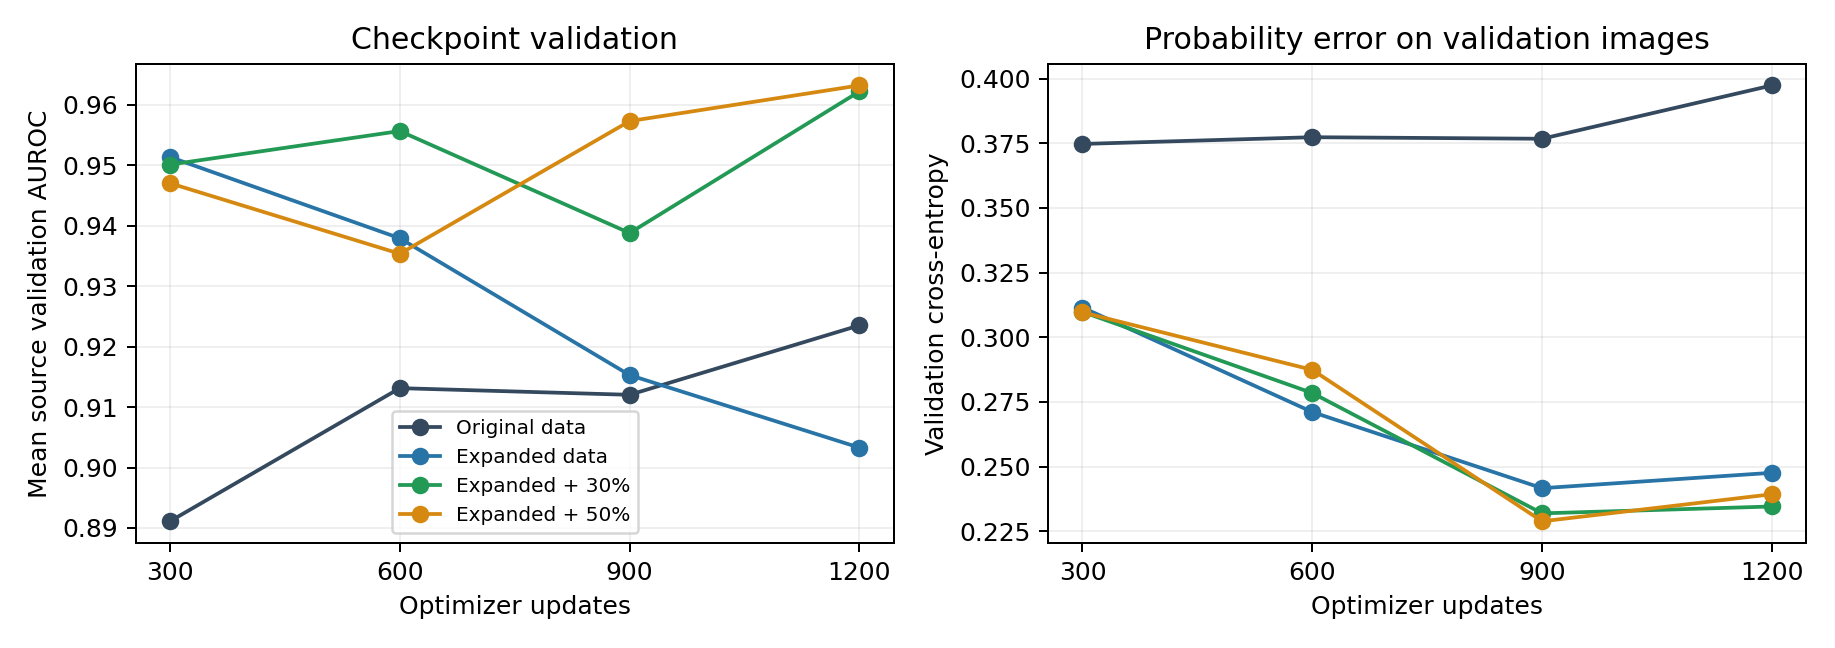
\includegraphics[keepaspectratio,alt={相同更新预算下的验证结果}]{training-curves.png}}
\caption{相同更新预算下的验证结果}
\end{figure}

图2左侧为来源AUROC平均值，右侧为全验证图像的交叉熵，即模型为错误答案给出高置信度时产生的概率误差。曲线节点是300、600、900和1,200次更新，表中权重选自这些节点，扩展无退化组选中第300次更新，其余组选中第1,200次更新。

\subsection{规则开发图像上的实际表现}\label{ux89c4ux5219ux5f00ux53d1ux56feux50cfux4e0aux7684ux5b9eux9645ux8868ux73b0}

下表使用每组已选权重，在相同原图上计算来源AUROC。规则开发集用于本轮训练后的分析。完整结果还包括AUPRC（精确率与召回率曲线下面积）、Brier分数（预测概率与0／1标签的平均平方误差）及校准误差。AUPRC受阳性比例影响，适合同一来源内比较；Brier分数越低，概率误差越小。

\Needspace{12\baselineskip}
\begin{longtable}[]{@{}lrrrr@{}}
\toprule\noalign{}
来源（开发图像／正例） & 原数据 & 扩展数据 & 30\%退化 & 50\%退化 \\
\midrule\noalign{}
\endhead
\bottomrule\noalign{}
\endlastfoot
AIROGS (773/380) & 0.9687 & 0.9374 & 0.9583 & 0.9593 \\
ODIR (305/28) & 0.9712 & 0.9323 & 0.9281 & 0.9404 \\
Kaggle (142/95) & 0.9830 & 0.9698 & 0.9742 & 0.9718 \\
LAG (481/169) & 0.9465 & 0.9750 & 0.9844 & 0.9832 \\
KEH (153/75) & 0.6627 & 0.9212 & 0.9321 & 0.9368 \\
BEH (33/8) & 0.9100 & 0.9050 & 0.8900 & 0.9100 \\
FIVES (27/13) & 0.8736 & 0.9341 & 0.9560 & 0.9505 \\
\end{longtable}

各组另按本来源验证阴性分数的第95百分位确定阈值，严格高于阈值才判为阳性。下表报告这些阈值在规则开发集上的敏感度和特异度，便于区分正例检出改善与整体分数上移；95\%是验证集上的目标，表中开发集特异度由新的病例分数决定。FIVES只有14张验证阴性，因此该规则在验证集选择最大阴性分数，达到100\%验证特异度。

\Needspace{12\baselineskip}
\begin{longtable}[]{@{}
  >{\raggedright\arraybackslash}p{(\linewidth - 8\tabcolsep) * \real{0.1579}}
  >{\raggedleft\arraybackslash}p{(\linewidth - 8\tabcolsep) * \real{0.2105}}
  >{\raggedleft\arraybackslash}p{(\linewidth - 8\tabcolsep) * \real{0.2105}}
  >{\raggedleft\arraybackslash}p{(\linewidth - 8\tabcolsep) * \real{0.2105}}
  >{\raggedleft\arraybackslash}p{(\linewidth - 8\tabcolsep) * \real{0.2105}}@{}}
\toprule\noalign{}
\begin{minipage}[b]{\linewidth}\raggedright
来源
\end{minipage} & \begin{minipage}[b]{\linewidth}\raggedleft
原数据：敏感度／特异度
\end{minipage} & \begin{minipage}[b]{\linewidth}\raggedleft
扩展数据
\end{minipage} & \begin{minipage}[b]{\linewidth}\raggedleft
30\%退化
\end{minipage} & \begin{minipage}[b]{\linewidth}\raggedleft
50\%退化
\end{minipage} \\
\midrule\noalign{}
\endhead
\bottomrule\noalign{}
\endlastfoot
ODIR & 71.4\% / 96.4\% & 42.9\% / 97.1\% & 53.6\% / 96.0\% & 53.6\% /
96.4\% \\
AIROGS & 84.2\% / 93.6\% & 71.3\% / 93.9\% & 78.2\% / 94.1\% & 76.3\% /
94.9\% \\
FIVES & 61.5\% / 92.9\% & 61.5\% / 100.0\% & 76.9\% / 92.9\% & 92.3\% /
78.6\% \\
\end{longtable}

MSHF入选49张图全部为正例，没有同来源阴性可估计特异度。MSHF结果因此报告阳性检出；FIVES同时报告阳性检出和阴性误报。

\begin{figure}[H]
\centering
\pandocbounded{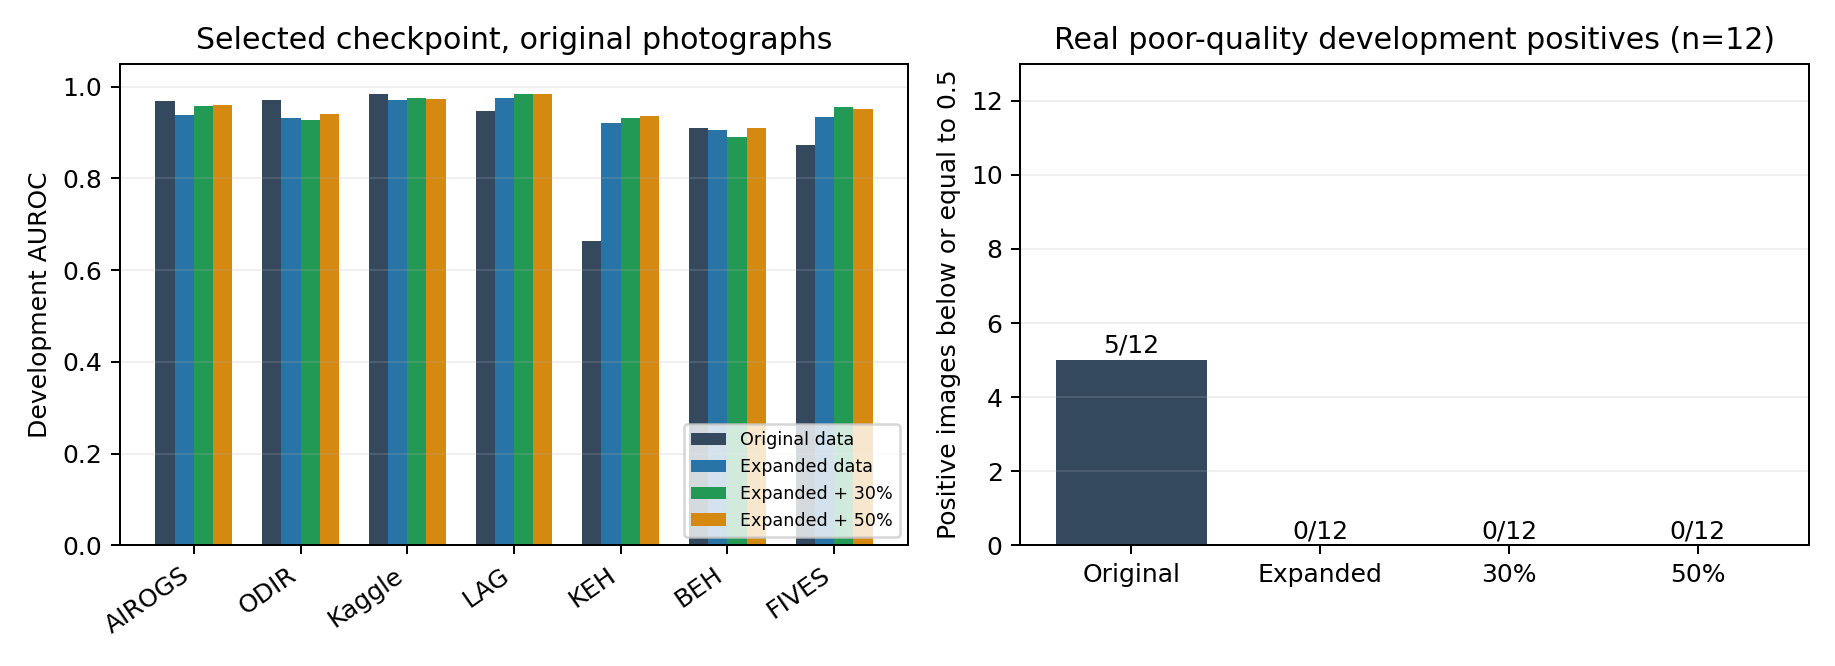
\includegraphics[keepaspectratio,alt={原图排序和真实低质量正例漏诊}]{development-results.png}}
\caption{原图排序和真实低质量正例漏诊}
\end{figure}

图3左侧比较七个主要来源的排序表现，右侧给出12张真实低质量正例的漏诊数量。0.5用于统一展示，来源验证阈值的结果见前表。12张低质量阳性由FIVES
7张和MSHF
5张组成，合计数描述这组固定开发照片。项目分类阈值及人工复核规则将在后续开发中确定。

\Needspace{12\baselineskip}
\begin{longtable}[]{@{}lrr@{}}
\toprule\noalign{}
对照（后者减前者） & 敏感度变化（百分点） & 关联组重抽样95\%区间 \\
\midrule\noalign{}
\endhead
\bottomrule\noalign{}
\endlastfoot
扩展数据 − 原数据 & +41.7 & {[}+16.7, +66.7{]} \\
30\%退化 − 扩展数据 & +0.0 & {[}+0.0, +0.0{]} \\
50\%退化 − 扩展数据 & +0.0 & {[}+0.0, +0.0{]} \\
\end{longtable}

区间按患者／图像关联组进行2,000次配对重抽样，比较同一张照片在两组模型中的阈值判断。本轮使用一个训练种子和12张正例，区间描述病例抽样变化。退化组与扩展无退化组在这12张上的判断完全一致，因此抽样差异区间为零；新病例上的差异仍需更大的真实质量样本评价。

另外按图像身份哈希选择同一批384张规则开发原图，其中146张正例、238张阴性，分别施加参考512像素视野半径2的失焦和曝光乘数0.70。表中每格是漏诊数量／误报数量，分别基于146张正例和238张阴性，以0.5为展示阈值；每张原图及其两个变体属于同一个病例观察。

\Needspace{12\baselineskip}
\begin{longtable}[]{@{}lrrrr@{}}
\toprule\noalign{}
条件 & 原数据：漏诊／误报 & 扩展数据 & 30\%退化 & 50\%退化 \\
\midrule\noalign{}
\endhead
\bottomrule\noalign{}
\endlastfoot
原图 & 30 / 16 & 28 / 20 & 21 / 13 & 23 / 14 \\
轻度失焦 & 55 / 10 & 3 / 104 & 36 / 23 & 28 / 19 \\
曝光乘数0.70 & 39 / 13 & 23 / 28 & 26 / 17 & 29 / 18 \\
\end{longtable}

扩展无退化组在失焦正例上漏诊3/146张，同时误报104/238张阴性，显示模糊图分数整体上移。30\%和50\%退化组的误报分别降为23/238和19/238，漏诊增加为36/146和28/146。真实低质量阳性结果见前表；真实低质量阴性是下一轮的补充重点。PAPILA、ACRIMA、HYGD及其余保留测试集将在模型和复核规则确定后评价。

\subsection{模型选择的补充检查}\label{ux6a21ux578bux9009ux62e9ux7684ux8865ux5145ux68c0ux67e5}

训练过程中，HRF仅4张验证图的一次排序变化就会改变来源AUROC平均值，使扩展数据组选中了第300次更新的权重。针对这个已观察到的问题，本次增加预算结束权重的开发评价，直接比较四组第1,200次更新，不改动原选模规则或选中权重。以下结果均来自同一规则开发集。

\Needspace{12\baselineskip}
\begin{longtable}[]{@{}
  >{\raggedright\arraybackslash}p{(\linewidth - 10\tabcolsep) * \real{0.1304}}
  >{\raggedleft\arraybackslash}p{(\linewidth - 10\tabcolsep) * \real{0.1739}}
  >{\raggedleft\arraybackslash}p{(\linewidth - 10\tabcolsep) * \real{0.1739}}
  >{\raggedleft\arraybackslash}p{(\linewidth - 10\tabcolsep) * \real{0.1739}}
  >{\raggedleft\arraybackslash}p{(\linewidth - 10\tabcolsep) * \real{0.1739}}
  >{\raggedleft\arraybackslash}p{(\linewidth - 10\tabcolsep) * \real{0.1739}}@{}}
\toprule\noalign{}
\begin{minipage}[b]{\linewidth}\raggedright
方案（第1,200次更新）
\end{minipage} & \begin{minipage}[b]{\linewidth}\raggedleft
ODIR AUROC
\end{minipage} & \begin{minipage}[b]{\linewidth}\raggedleft
AIROGS AUROC
\end{minipage} & \begin{minipage}[b]{\linewidth}\raggedleft
KEH AUROC
\end{minipage} & \begin{minipage}[b]{\linewidth}\raggedleft
真实低质量漏诊
\end{minipage} & \begin{minipage}[b]{\linewidth}\raggedleft
合成失焦误报
\end{minipage} \\
\midrule\noalign{}
\endhead
\bottomrule\noalign{}
\endlastfoot
原数据 & 0.9712 & 0.9687 & 0.6627 & 5/12 & 10/238 \\
扩展数据 & 0.9315 & 0.9551 & 0.9333 & 0/12 & 68/238 \\
扩展＋30\%退化 & 0.9281 & 0.9583 & 0.9321 & 0/12 & 23/238 \\
扩展＋50\%退化 & 0.9404 & 0.9593 & 0.9368 & 0/12 & 19/238 \\
\end{longtable}

该表与前面的选中权重结果分开保存，用于判断原有来源排序的下降有多少来自较早选模。下一轮应预先以具有足够正负例的主要来源设定选择标准，增加随机种子和更新预算，保留原图与真实低质量病例的检出、特异度和概率误差，然后锁定分类阈值及质量引导复核规则。

本轮数据扩展的主要观察为：同一1,200次更新预算下，KEH开发AUROC从0.6627提高到0.9333，真实低质量开发正例的展示阈值漏诊从5/12减少到0/12。50\%退化将扩展模型的ODIR
AUROC从0.9315提高到0.9404，仍低于原数据对照的0.9712；三个扩展组均检出这12张低质量阳性。下一轮需处理原有来源的排序和阈值表现，并补充真实低质量病例比较退化的额外效果。

同预算的合成失焦评价中，50\%退化将扩展原图模型的阴性误报从68/238降低到19/238，正例漏诊从18/146变为28/146。该变化明确呈现了误报减少与漏诊增加的关系；下一轮将结合真实低质量阴性，评价固定筛查阈值下的表现。

\subsection{代码、证据和复现}\label{ux4ee3ux7801ux8bc1ux636eux548cux590dux73b0}

\href{data-audit.zh.md}{数据整合审计} ·
\href{degradation-audit.zh.md}{退化方法审计} ·
\href{../../../../data/prepared/expanded_20261113/cohort_verification.json}{冻结清单核验}
·
\href{../../../../runs/expanded_20261113/comparison.json}{完整对照结果}
·
\href{../../../../runs/expanded_20261113/budget_end_comparison.json}{预算结束权重检查}
· \href{../../../../configs/expanded_20261113/}{四组配置} ·
\href{../../../../tools/start_expansion_experiments_20261113.ps1}{启动脚本}

已完成的目录保留best.pt、last.pt、逐步损失、验证曲线、原图和压力版本的开发预测，以及退化参数记录。配置、初始化、数据清单、发布信息和训练模块共同绑定到权重指纹；恢复时检查一致性。重新运行启动脚本会核查已完成预算，保留本轮产物。更改训练预算或设计时建立新配置和输出目录。

\end{document}
